\section{Results}

In this section we present the results of our system. We use three locomotion tasks to test our system: The robot rises from a leaning, sitting or kneeling position to an erect stance. Please watch the accompanying video for the robot performance in the simulation and in the real world.

\subsection{Experiment Setup}

We choose BIOLOID GP as our robot platform. BIOLOID GP is a humanoid robot that consists of 18 degrees of freedom powered by Dynamixel AX-12/AX-18 servos. The communication between the PC and the robot is through a serial port. To control the robot, a master program on the PC writes the desired pose $\bar{\mathbf{q}}$ to the serial port that is connected to the robot. A slave program that runs on the robot's onboard microprocessor listens to this port and sends the desired joint angle to each actuator. At the same time, the robot performance data $\tilde{\mathbf{x}}$ is measured and sent back to the computer. We use onboard rotary encoders to measure joint angles and a VICON motion capture system to measure the global position and orientation of the robot's torso. The average latency of the whole control loop on our robot is 16ms. It is measured by a timer in our program between the time that the program starts sending the actuator commands to the robot and the time that it finishes reading the sensor measurements from the robot.

\subsection{Implementation Details}

Our system was implemented in C++ and ran on a laptop with 2.6GHz quad-core CPU and 16GB of memory. We used DART to simulate the physics of the robot and its surrounding environments. We use 1ms as the time step in physical simulation. We only update the control signal every 16 time steps to better match our simulation with the actual latency. In controller optimization, we halve the size of the optimization problem by exploiting the symmetry of the motion. We find that all four tasks can be achieved with symmetric motions. Thus we constrain that the joint motions on the left bodies mirror those on the right bodies. In addition, we only search for the joint trajectories for the lower body. The CMA solvers in both controller optimization and simulation calibration use 32 samples per iteration and at most 50 iterations. We distribute the computation across all four cores on the CPU. It takes less than 15 minutes to find an optimal solution in controller optimization or simulation calibration.


\subsection{Rising from a Sitting Position}

\begin{figure*}[!t]
  \centering
  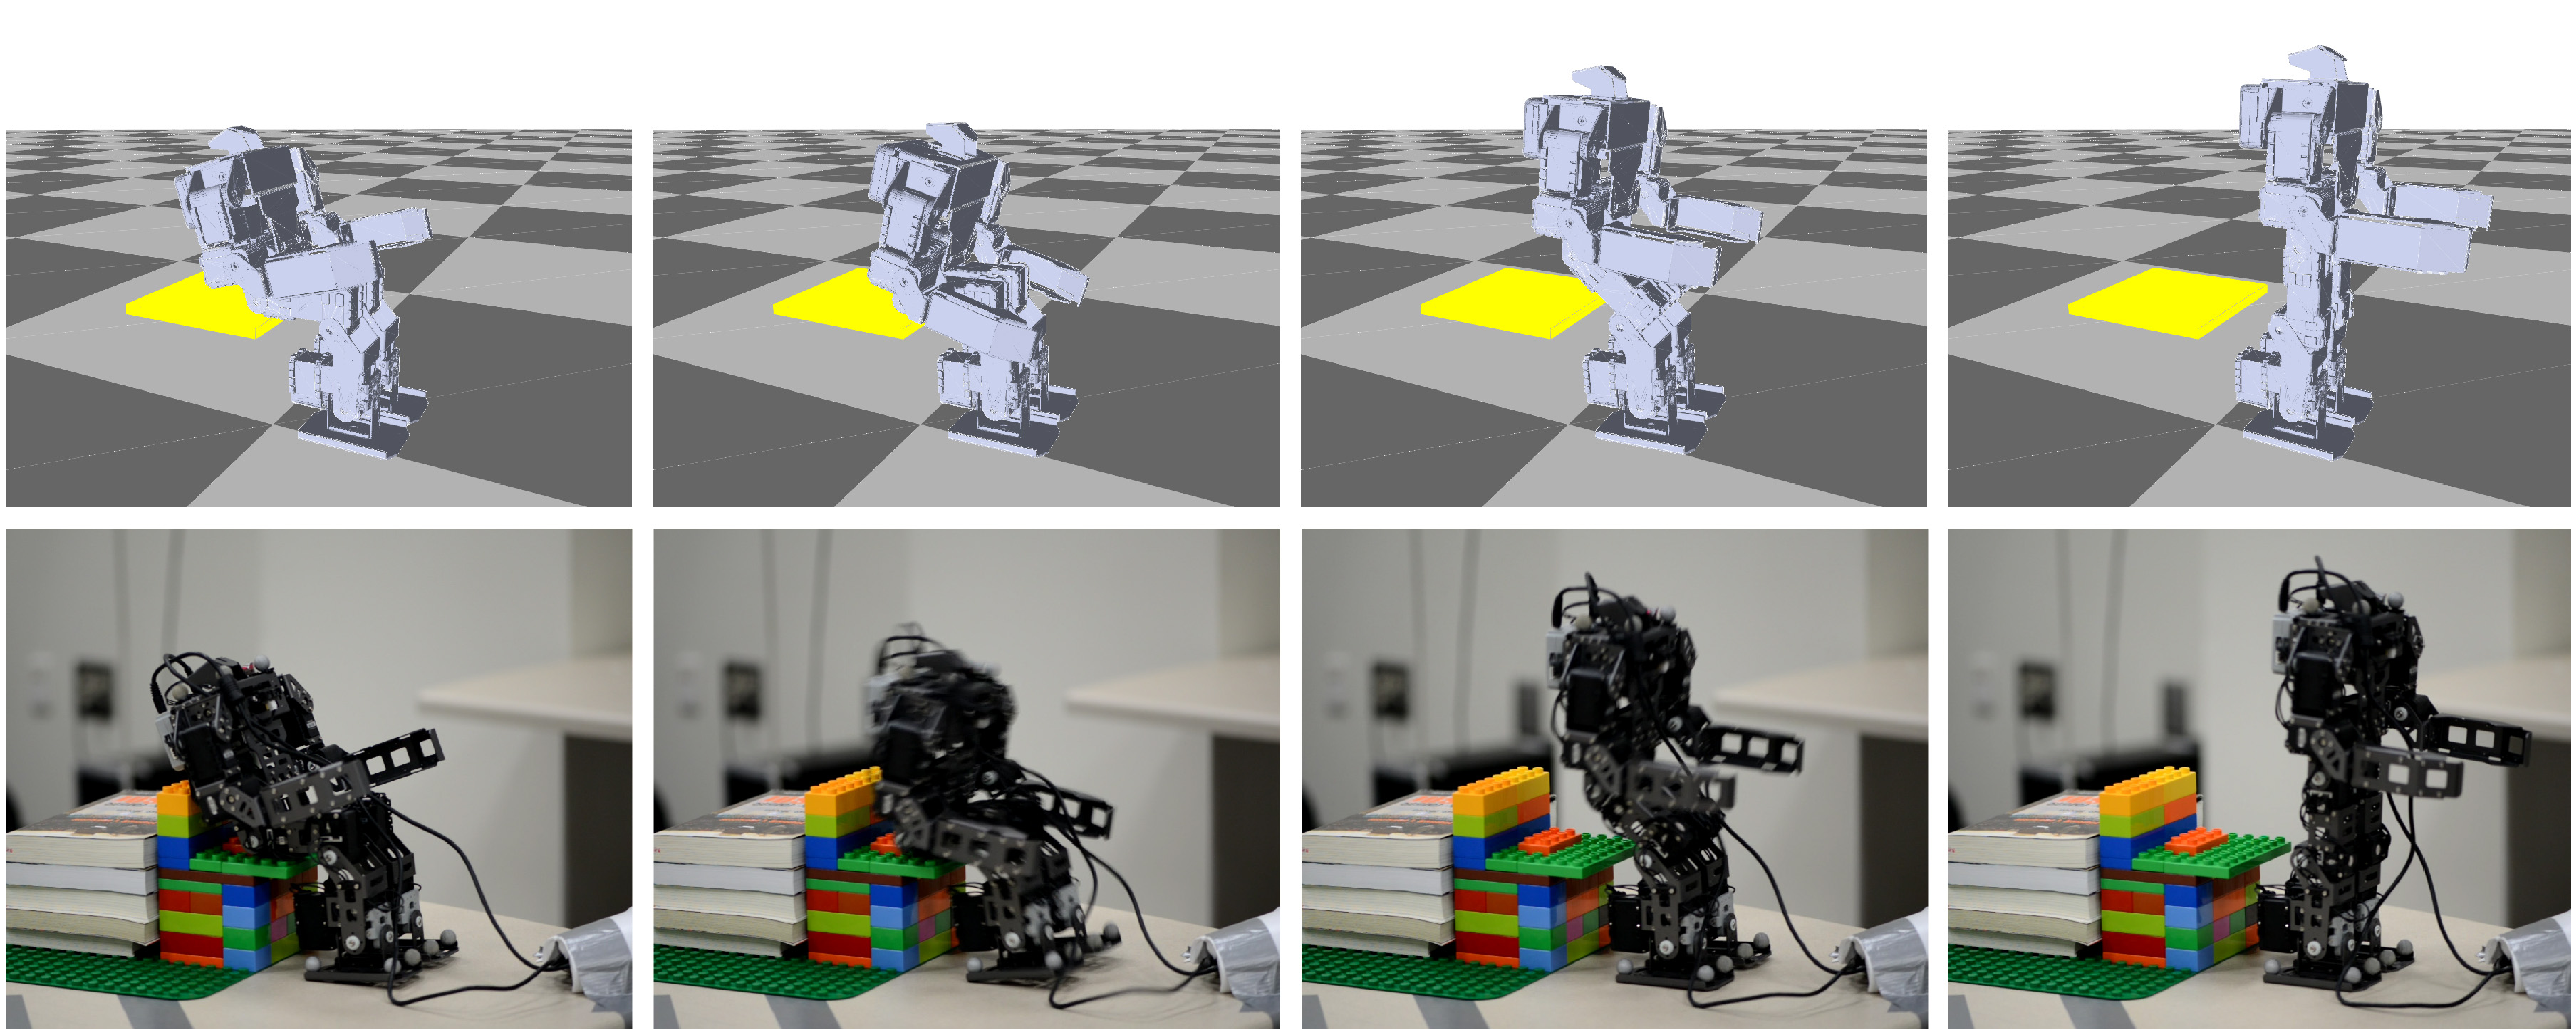
\includegraphics[width=\textwidth]{figures/sit2Stand}
  \caption{The results of the sit-to-stand task in the simulation and on the real robot.}
  \label{fig:sit2Stand}
\end{figure*}

The first task that we have tested is to rise from a sitting pose to a standing pose (Figure \ref{fig:sit2Stand}). The initial and final poses $q_0$ and $q_T$ are shown in the leftmost and rightmost images in Figure \ref{fig:sit2Stand}. We parameterize the controller with three keyframes $q_0$, $q_1$ and $q_T$. In addition to $q_0$ and $q_T$ specified by the user, the controller optimization subsystem needs to search for the keyframe $q_1$, and the two time intervals $t_1$ and $t_2$ between the three keyframes. Note that we only change the joint angles of the hips and the knees and keep all other joints motionless throughout the entire motion.

We purposefully choose the initial pose that the legs of the robot extend forward and the projection of the robot's COM in the vertical direction falls far behind the contact points of the feet. If the robot simply extends the hips and the knees to stand up, it will fall backwards. Despite this challenging setup, our system successfully finds a controller that enables the robot to stand up in the simulation. Figure \ref{fig:sit2Stand} shows that the robot first builds up a forward momentum by quickly leaning its upper body to the front. It then starts to extend the hips and the knees at the moment when the COM is approaching the boundary of the support polygon spanned by the feet. This effective standing-up strategy is found automatically by the controller optimization subsystem.

When applying this controller to the real robot, we are surprised to find that it works directly, without the need of simulation calibration. The robot stands up from a chair in the same way as its simulated counterpart does in the virtual world. It shows that the Reality Gap is not always a problem. In some tasks, the stability region of a controller is so large that it can make the discrepancy between the virtual and the real world less critical.

\subsection{Rising from a Leaning Position}

\begin{figure}[!t]
  \centering
  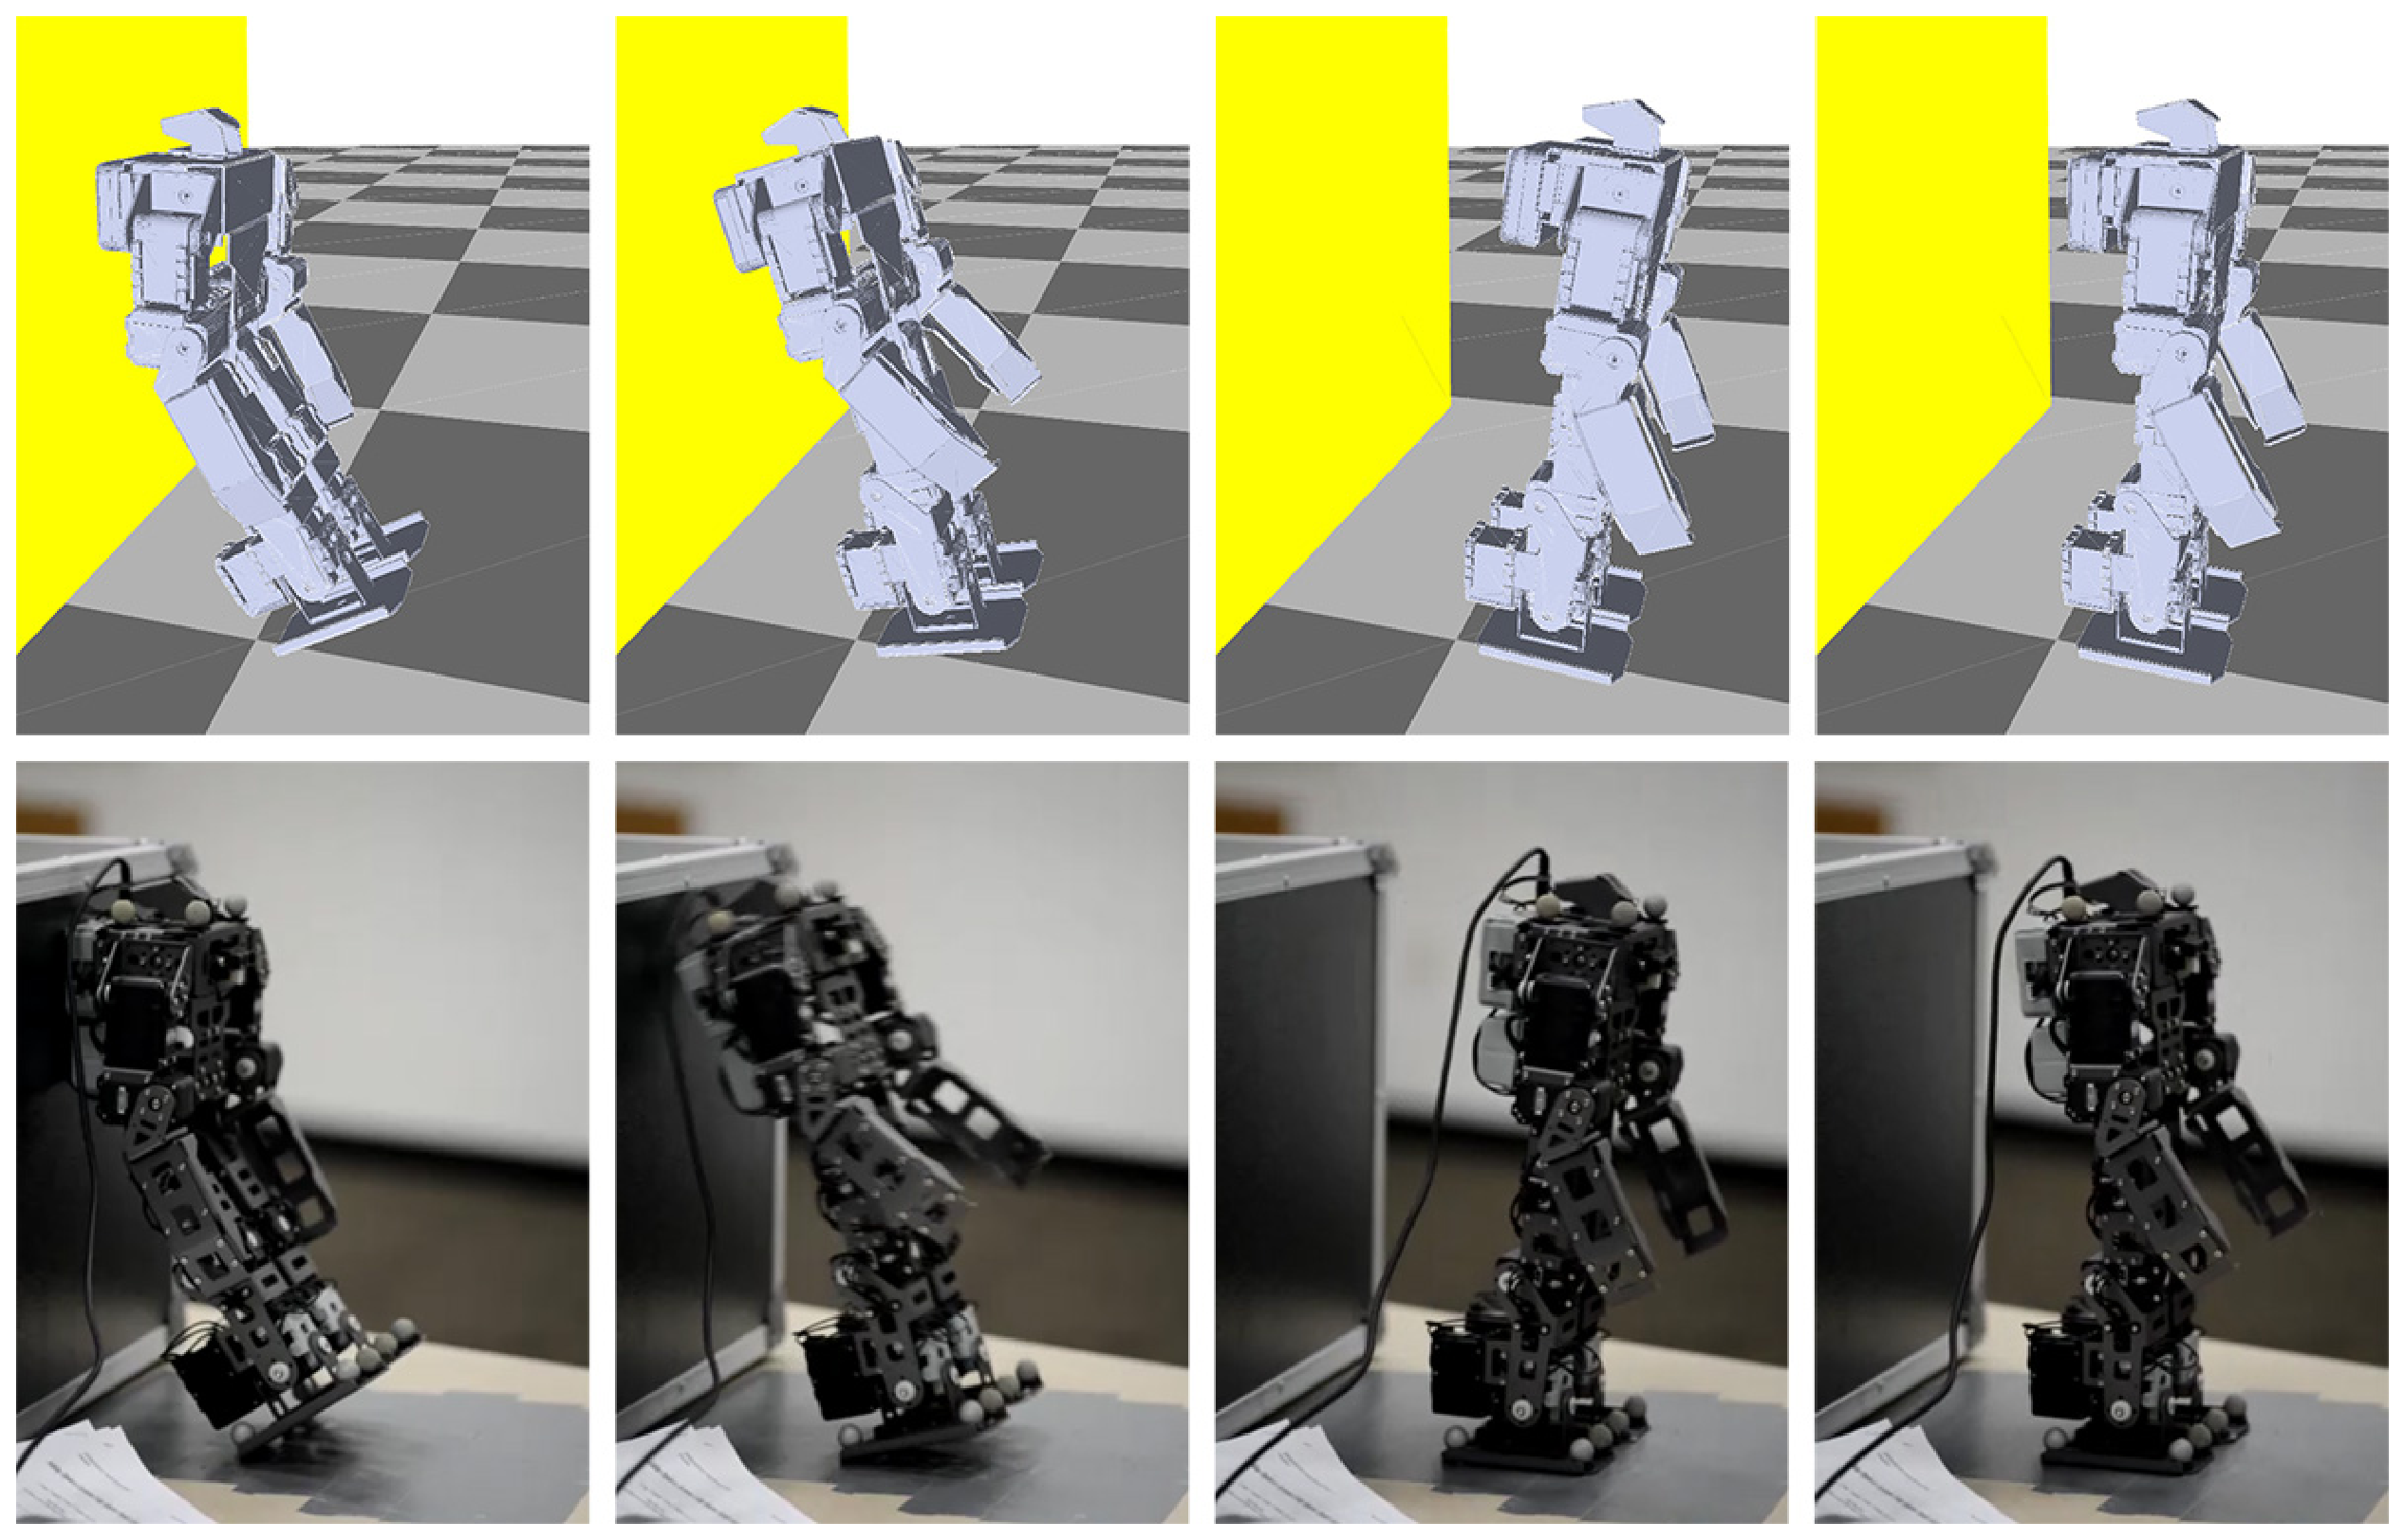
\includegraphics[width=0.5\textwidth]{figures/lean2Stand}
  \caption{The results of the lean-to-stand task in the simulation and on the real robot.}
  \label{fig:lean2Stand}
\end{figure}

In this task, the robot needs to rise from leaning on the wall (the leftmost image in Figure \ref{fig:lean2Stand}) to a standing position (the rightmost image in Figure \ref{fig:lean2Stand}). In the initial configuration, the hip joints are bent and they are straightened out in the final configuation while all other joints do not move. The initial and the final poses are the only two keyframes for this task.

\begin{figure}[!t]
  \centering
  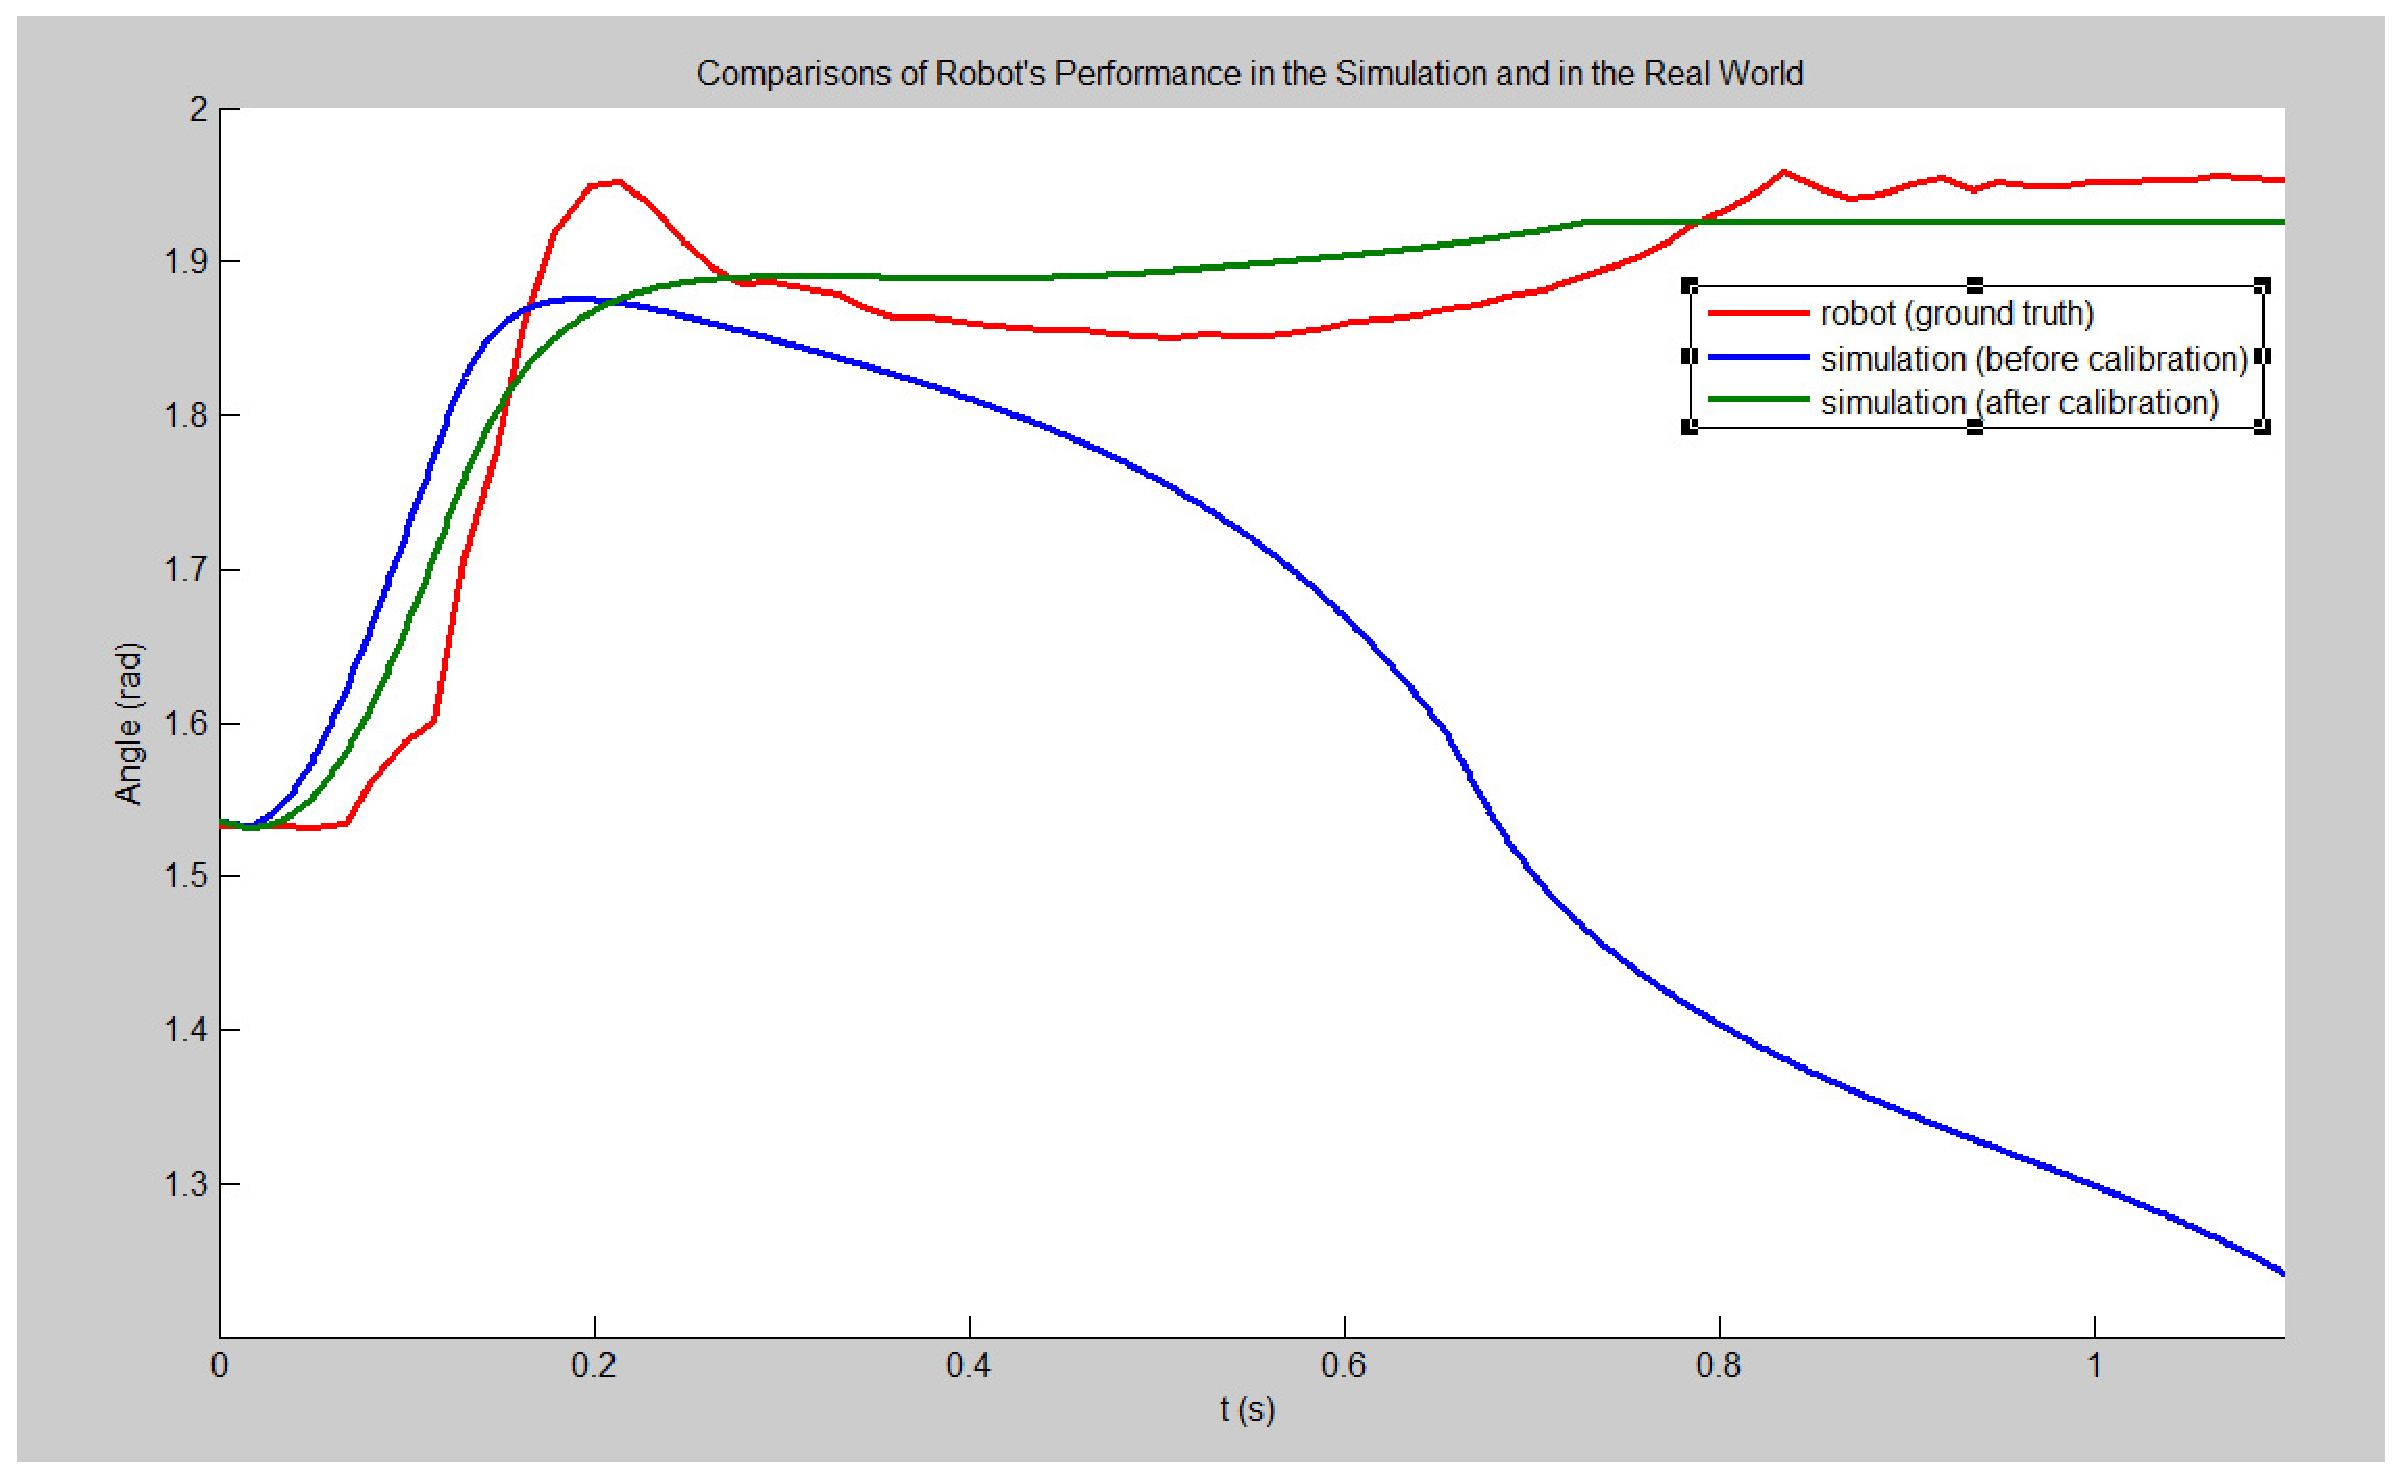
\includegraphics[width=0.4\textwidth]{figures/simRobotCompare}
  \caption{Comparisons of the robot's global orientation over time in the simulation (before/after calibration) and in the real environment.}
  \label{fig:simRobotCompare}
\end{figure}


The goal of controller optimization is to find an appropriate time interval $T$ between these two keyframes. If the time inteval is too long, the robot moves slowly, and cannot accumulate enough momentum to rise up. If this time inteval is too short, the robot move abruptly, which will cause the upper body to bounce off the wall too quickly and fall forward. Without simulation calibration, the optimization cannot find a working controller for this task. The robot cannot rise up when $T\leq 0.10s$ and overshoots when $T > 0.10s$. According to the objective function value, the optimal controller, which still fails the task, uses $T=0.11s$ to move from the initial to the final pose. Using this controller, the robot rises up too quickly and falls forward in the simulation. When we apply this controller to the real robot, we find that its performance in the real world differs drastically from that in the simulation. Rather than falling forward, the robot in the real world cannot rise up. The red and blue curves in Figure \ref{fig:simRobotCompare} show the the trajectories of the robot's global orientation in the simulation and in the real world. After one iteration of simulation calibration, the discrepancy is greatly reduced (Figure \ref{fig:simRobotCompare} green curve). We optimize the controller again in the calibrated simulator. This time, the optimal controller works both in the simulated and in the real environment.

\begin{figure}[!t]
  \centering
  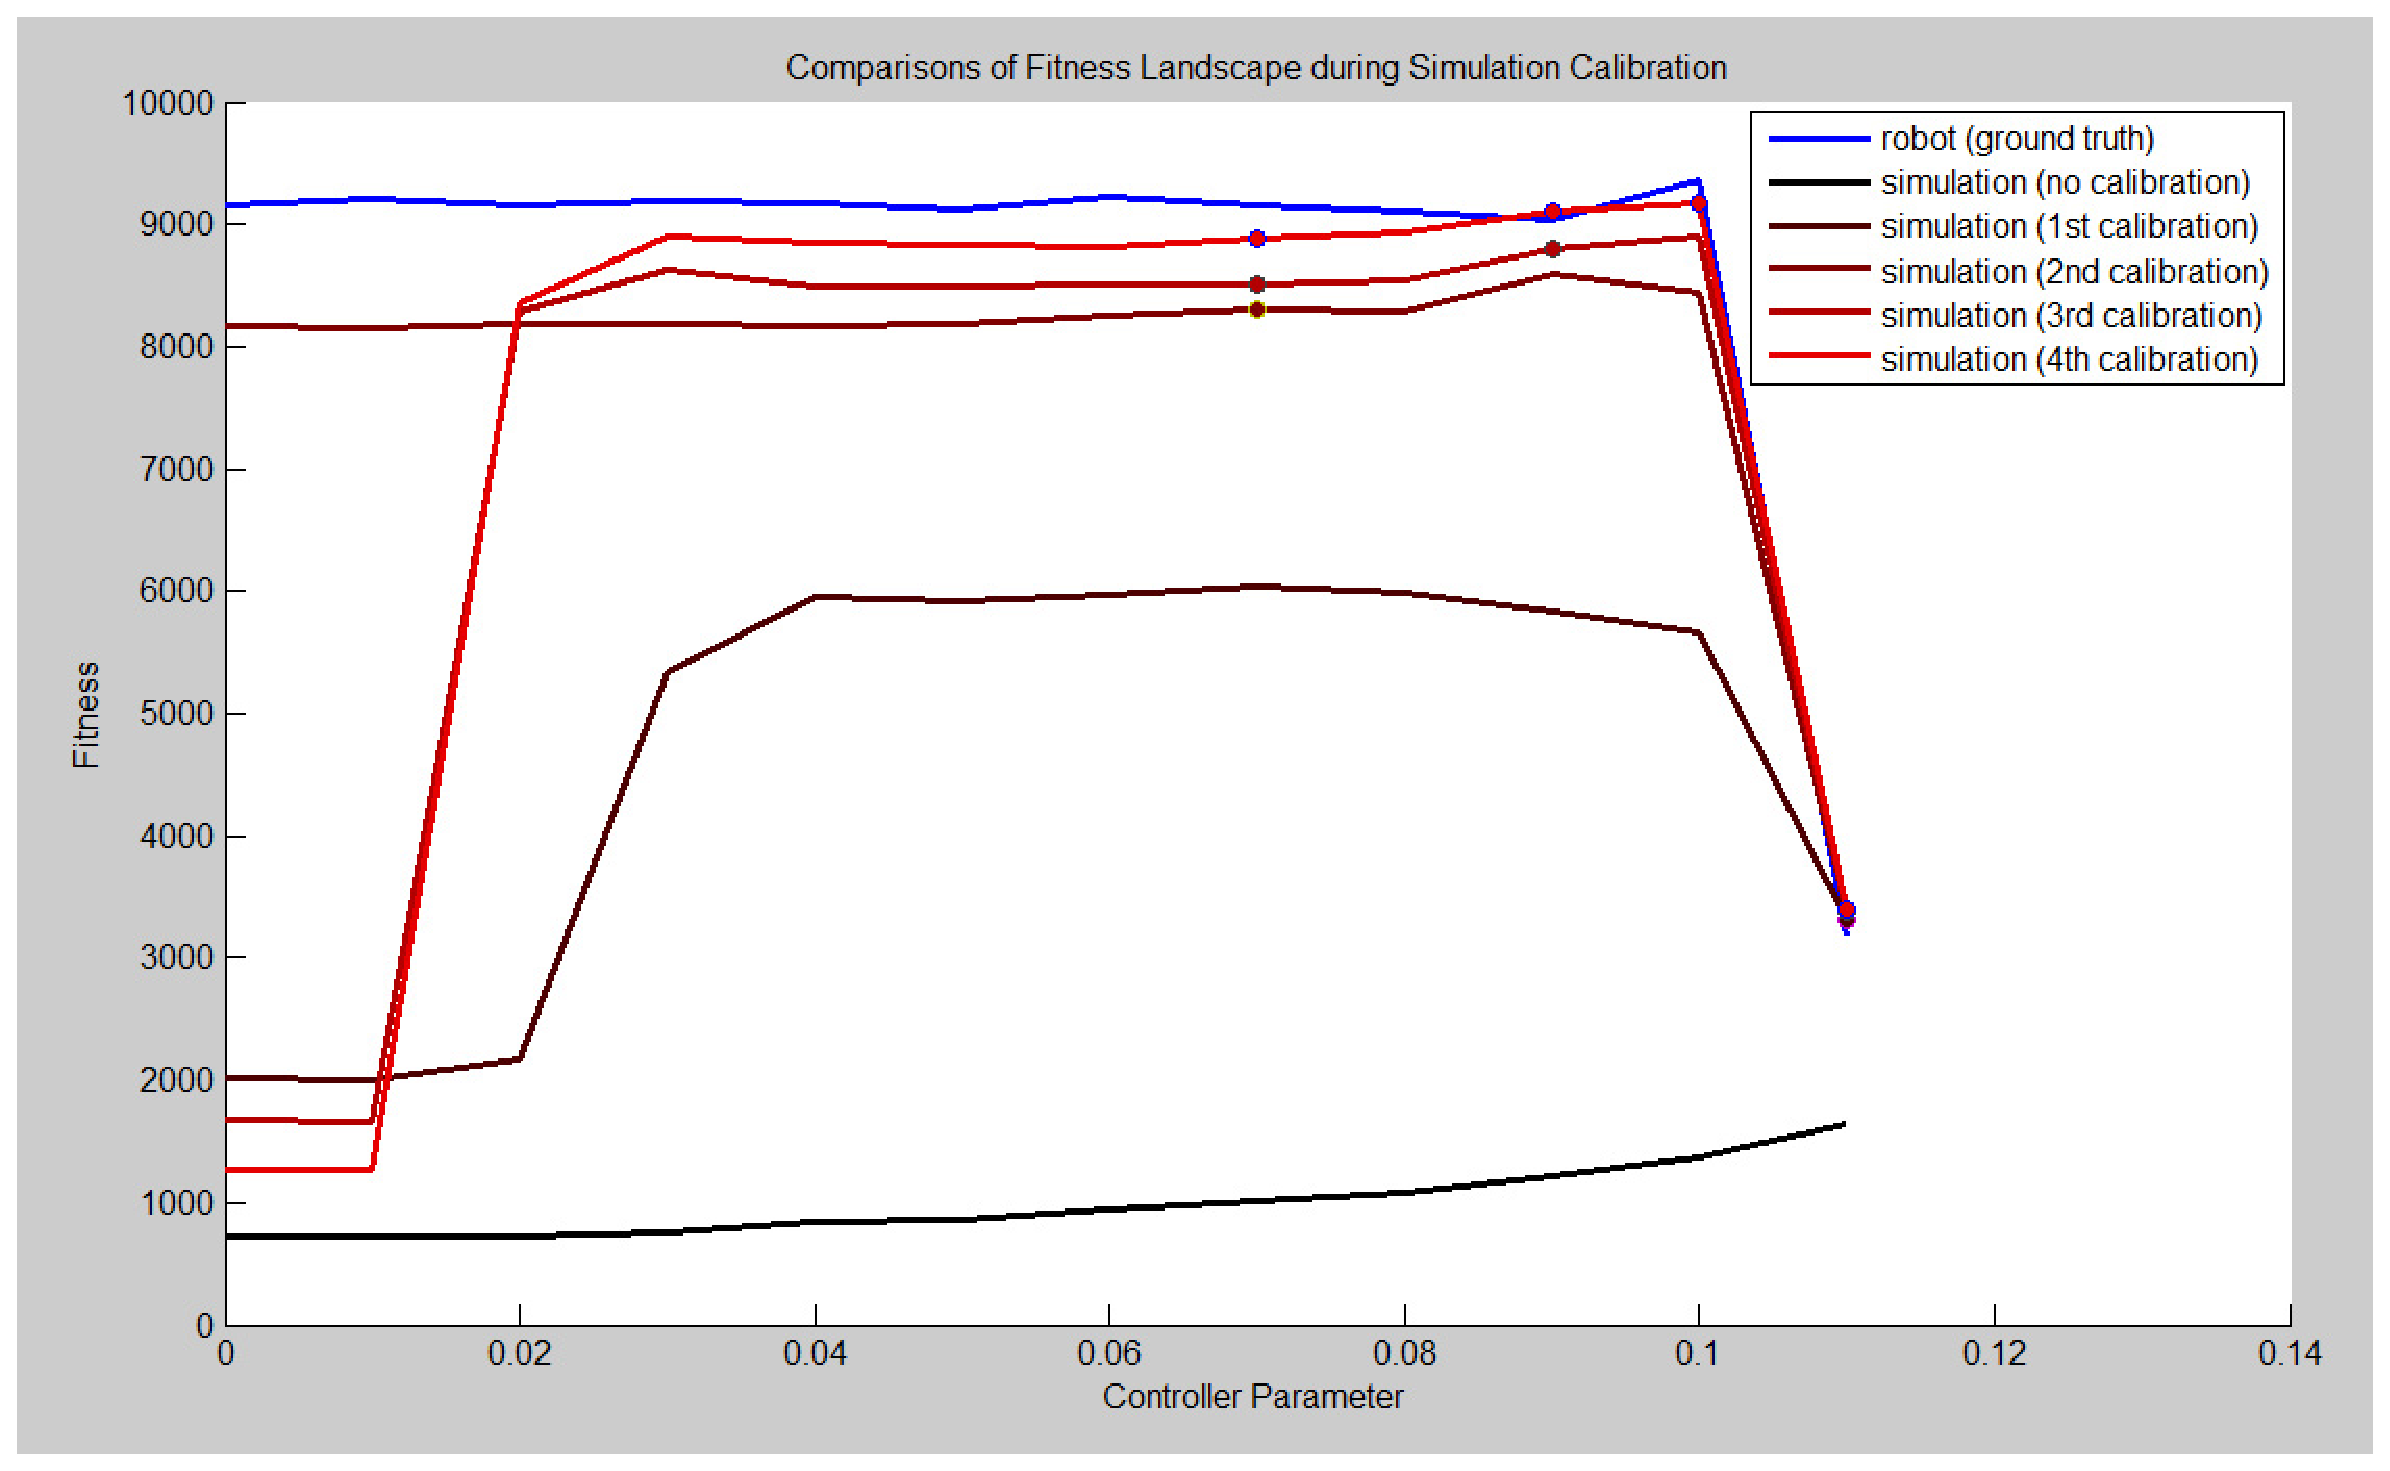
\includegraphics[width=0.4\textwidth]{figures/fitnessLandscape}
  \caption{Comparisons of the fitness functions as more and more iterations of simulation calibration are performed.}
  \label{fig:fitnessLandscape}
\end{figure}

We successfully crosses the Reality Gap using only one iteration of simulation calibration. To better understand how the Reality Gap is gradually narrowed by simulation calibration over multiple iterations, we perform an additional evaluation. Figure \ref{fig:fitnessLandscape} shows the fitness functions after different number of iterations of simulation calibration. The blue curve is the fitness function on the real robot by varying the control parameter $T$ in the range of $[0, 0.11]$. It serves as the ground truth. The fitness function stays at a high value when $T\in[0, 0.1]$, which means that the real robot can successfully rise if the controller uses less than 0.1s to change the pose from the initial to the final configuration. In contrast, without simulation calibration, the fitness function (lowest black curve) stays at a low value for the entire control space. In other words, no controller exists that can make the robot stand up in the simulation. The gap between the blue and the black curves is analogue to the Reality Gap. One iteration of system calibration brings the fitness function in the simulation towards the ground truth. As more iterations are performed, the fitness function in the simulation (brown and red curves) gradually approaches the ground truth, and the Reality Gap is narrowed in this process. Note that a large discrepancy still exists in the region of the parameter space where $T<0.02s$. This is probably caused by two reasons. First, in the region of $T<0.02s$, the torque output of the servo is at its limit but the torque limit is not considered in simulation calibration. Second, the controllers and the data (the red circles in Figure \ref{fig:fitnessLandscape}) that we use in simulation calibration concentrate on the right half of the parameter space, which makes it difficult to generalize to a region where the data is scarce ($T<0.02$). However, this could be beneficial in many applications because the computational resource is focused at the important regions near the successful controllers.

\subsection{Rising from a Kneeling Position}

\begin{figure*}[!t]
  \centering
  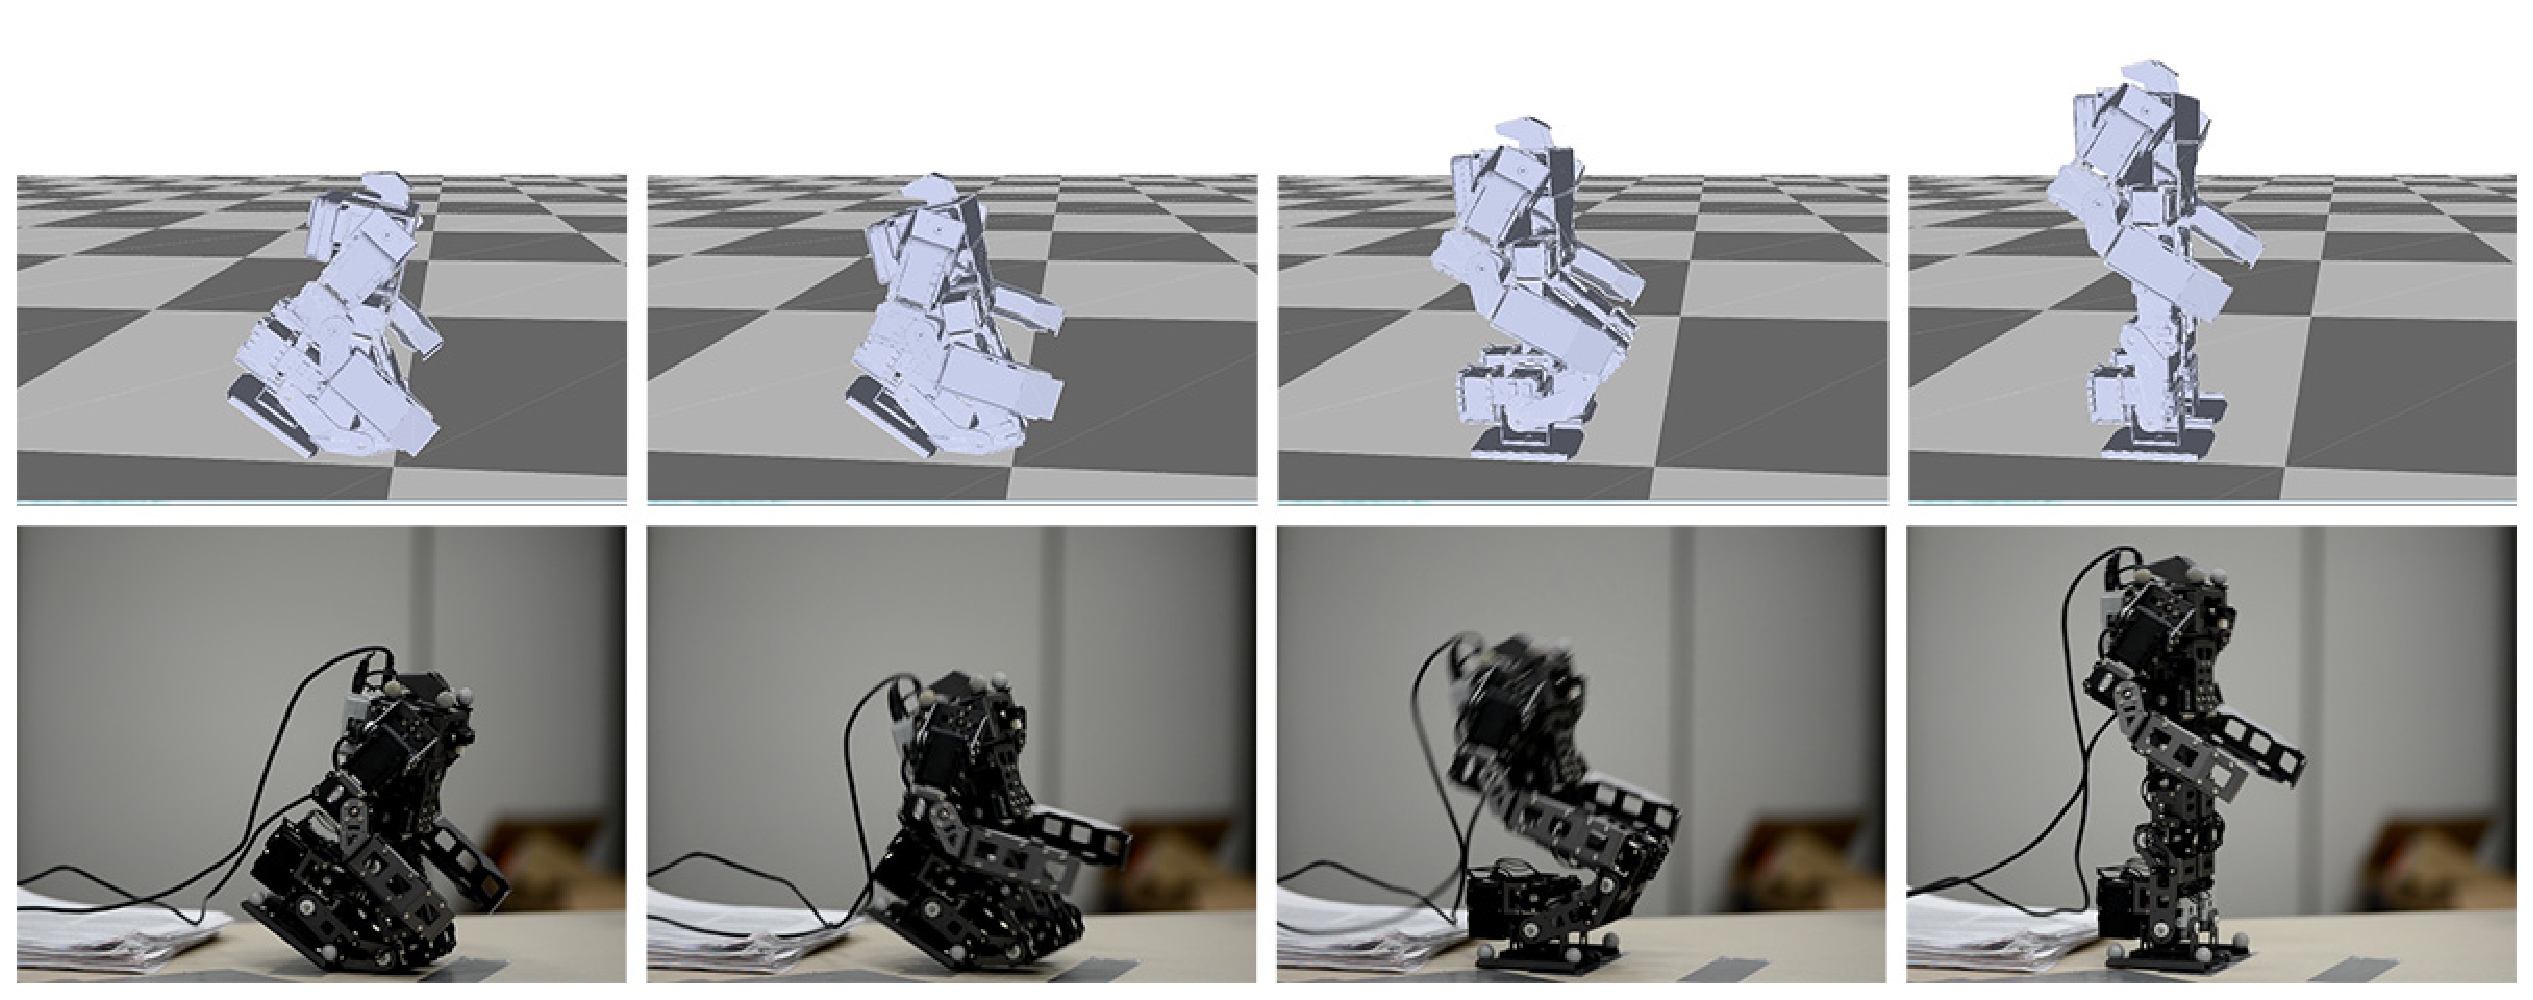
\includegraphics[width=\textwidth]{figures/kneel2Stand}
  \caption{The results of the kneel-to-stand task in the simulation and on the real robot.}
  \label{fig:kneel2Stand}
\end{figure*}

Figure \ref{fig:kneel2Stand} shows that the robot stands up from a kneeling pose. Between the user-specified initial and final poses, the controller consists of two additional keyframes. The optimization needs to search for these keyframes and the time intevals between adjacent keyframes. Similar to other examples, we only allow the joints on the lower body of the robot to move. The controller optimized in the simulation demonstrates an agile getting-up motion: The robot first leans its upper-body backwards. As its COM is moving to the back, it quickly bends the hip, flexes its ankels and stands up. This entire motion resembles one of the most agile ways that we human get up from a kneeling position when we do not use our hands for additional support. Although this controller works perfectly in the simulation, the robot falls backward in the real world. After simulation calibration, the performance of the simulated robot comes closer to the real world scenario: The robot also falls backward in the simulation. Using the calibrated simulator, we optimize a new controller, with which the robot can successfully stand up from the kneeling position in the real world (Figure \ref{fig:kneel2Stand}).
